% !TEX TS-program = lualatex
\documentclass[11pt,a4paper]{article}

% Layout & language
\usepackage[a4paper,margin=2.2cm]{geometry}
\usepackage[english]{babel}
\usepackage{lmodern}
\usepackage{microtype}

% Math
\usepackage{amsmath,amssymb,mathtools}
\usepackage{siunitx}
\usepackage{bm}
\usepackage{upgreek}

% Links & refs
\usepackage[hidelinks]{hyperref}
\usepackage[nameinlink,capitalise]{cleveref}

% TikZ + pgfplots
\usepackage{tikz}
\usetikzlibrary{arrows.meta,positioning}
\usepackage{pgfplots}
\pgfplotsset{compat=1.18}

% Unicode em-dash mapping (if it appears)
\usepackage{newunicodechar}
\newunicodechar{—}{\textemdash{}}

% Macros
\newcommand{\sigP}{\sigma_{\mathrm P}}   % l_P t_P = \hbar G / c^4
\newcommand{\lP}{\ell_{\mathrm P}}
\newcommand{\tP}{t_{\mathrm P}}
\newcommand{\kappaE}{\kappa}             % 8\pi G / c^4
\newcommand{\cO}{\mathcal O}
\newcommand{\aO}{a_0}
\newcommand{\gN}{g_{\mathrm N}}
\newcommand{\gs}{g_{\sigma}}
\newcommand{\PhiN}{\Phi_{\mathrm N}}
\newcommand{\PhiS}{\Phi_{\sigma}}

\title{\textbf{MOND-like Law from Source-Smeared GR \\(Einstein Unchanged)}\\
\large Geometry-Averaged GR from the Planck Two-Measure and Consistency with Early-Universe Probes}
\author{\textbf{Adrian Zander}}
\date{\today}

\begin{document}
\maketitle

\section*{Status / Einordnung}
\noindent\textbf{Document type:} Working Paper (phenomenology derivation draft)\\
\textbf{Claim level:} Testable theoretical hypothesis. Derivations and assumptions should be treated as draft-level until fully checked and compared against standard benchmarks and observational fits.\\
\textbf{Use:} Use for derivation review and falsifiable prediction design.


\begin{abstract}
We derive the MOND phenomenology from \emph{unchanged} Einstein equations by replacing the microscopic source $T_{\mu\nu}$ with a Lorentz-covariant average over the invariant two-measure $\sigP=\lP\tP=\hbar G/c^4$.
In thin, axisymmetric, weak-field disks the smeared Green function develops a logarithmic sector so that
\[
g_{\rm obs}(r)=\gN(r)+\sqrt{\gN(r)\,\aO},\qquad \gN=\frac{G M_b(r)}{r^2},
\]
with a single boundary constant
\[
\boxed{~\aO=\frac{c}{2\pi\,T}=\frac{c\,H_0}{2\pi}~}.
\]
This reproduces flat rotation curves, BTFR and the RAR without dark matter. Homogeneous FRW and high-acceleration epochs remain unmodified to leading order.
\end{abstract}

\section*{1. Einstein side unchanged; modified \emph{source}}
\[
G_{\mu\nu}[g]+\Lambda g_{\mu\nu}=\kappaE\,T_{\mu\nu},
\quad \kappaE=\frac{8\pi G}{c^4}.
\]
Introduce a Planck-covariant source average
\begin{equation}
\overline{T}_{\mu\nu}(x)=\!\int d^4y\,\sqrt{|g(y)|}\;K_{\sigP}(x,y)\;\Pi_{\mu}{}^{\mu'}(x,y)\Pi_{\nu}{}^{\nu'}(x,y)\;T_{\mu'\nu'}(y),
\label{eq:smear}
\end{equation}
with positive kernel $K_{\sigP}\!\ge0$ and parallel propagator $\Pi$. Local conservation holds up to $\cO(\sigP^2)$.
A minimal kernel based on Synge’s world function $\sigma(x,y)$ is
\begin{equation}
K_{\sigP}(x,y)=\frac{1}{(2\pi\sigP)^2}\exp\!\Big(-\frac{2\,\sigma(x,y)}{\sigP}\Big).
\label{eq:kernel}
\end{equation}

\section*{2. Why MOND-like scaling emerges (thin disks)}
In the weak-field limit ($g_{tt}=-1-2\Phi/c^2$) with a razor-thin, axisymmetric disk $\rho=\Sigma_b(R)\delta(z)$ the Green function acquires a logarithmic sector
\begin{equation}
\PhiS(R)=v_0^2\ln(R/R_0),\qquad \gs(R)=\partial_R\PhiS=\frac{v_0^2}{R}.
\label{eq:log}
\end{equation}
Defining $v_0^2=\sqrt{G M_b(R)\,\aO}$ gives
\begin{equation}
\boxed{~g_{\rm obs}= \gN + \sqrt{\gN\,\aO}~}.
\label{eq:gobs}
\end{equation}
This form matches BTFR and the RAR (BTFR \cite{McGaugh2012BTFR}; RAR \cite{McGaugh2016RAR}) and can be tested on SPARC \cite{Lelli2016SPARC}.

\paragraph{Plots.}
\begin{figure}[t]
\centering
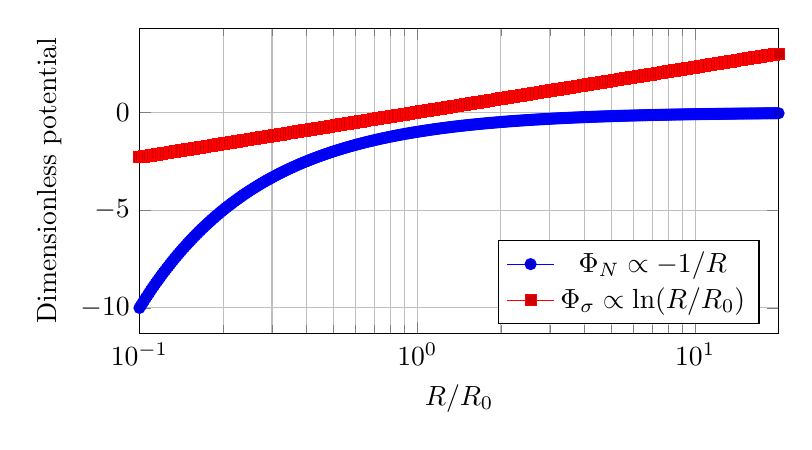
\begin{tikzpicture}
\begin{axis}[width=0.8\textwidth,height=0.45\textwidth,
xmin=0.1,xmax=20,xmode=log,
xlabel={$R/R_0$},ylabel={Dimensionless potential},
legend pos=south east,grid=both]
\addplot+[domain=0.1:20,samples=400] {-1/x};
\addlegendentry{$\Phi_N \propto -1/R$}
\addplot+[domain=0.1:20,samples=400] {ln(x)};
\addlegendentry{$\Phi_\sigma \propto \ln(R/R_0)$}
\end{axis}
\end{tikzpicture}
\caption{Newtonian vs. logarithmic potential (dimensionless).}
\end{figure}

\begin{figure}[t]
\centering
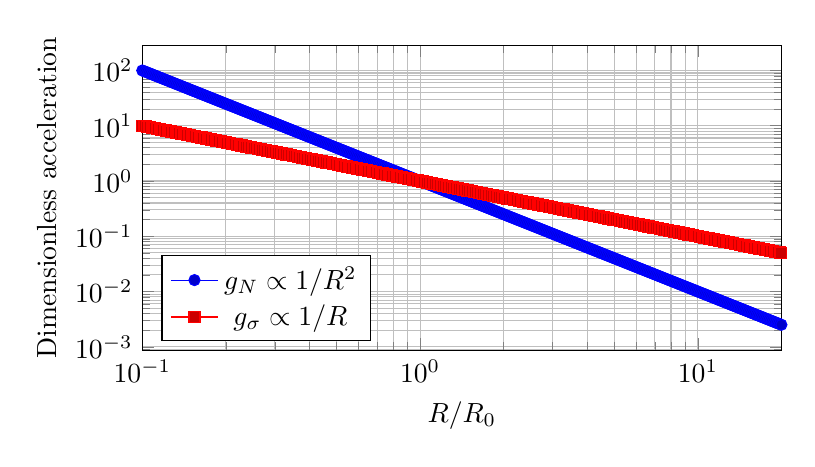
\begin{tikzpicture}
\begin{axis}[width=0.8\textwidth,height=0.45\textwidth,
xmin=0.1,xmax=20,xmode=log,ymode=log,
xlabel={$R/R_0$},ylabel={Dimensionless acceleration},
legend pos=south west,grid=both]
\addplot+[domain=0.1:20,samples=400] {1/x^2};
\addlegendentry{$g_N \propto 1/R^2$}
\addplot+[domain=0.1:20,samples=400] {1/x};
\addlegendentry{$g_\sigma \propto 1/R$}
\end{axis}
\end{tikzpicture}
\caption{Accelerations: Newton $1/R^2$ vs. log sector $1/R$.}
\end{figure}

\section*{3. Geometric origin of the factor $2\pi$}
In 2D, the Poisson Green’s function is $G_{2D}=(2\pi)^{-1}\ln r$ (contrast $G_{3D}=-(4\pi r)^{-1}$). A thin disk effectively samples this 2D sector, hence the $(2\pi)^{-1}$ normalization and $g\propto 1/R$.

\paragraph{Hierarchical dual network (pull/hold).}
\begin{figure}[t]
\centering
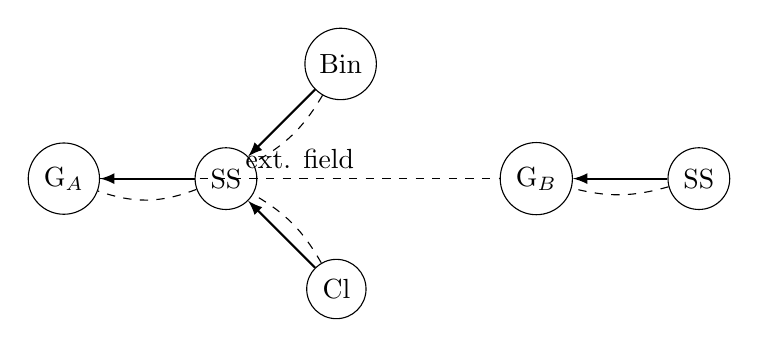
\begin{tikzpicture}[>=latex,node distance=1.2cm]
\tikzstyle{gal}=[circle,draw,minimum size=8mm]
\tikzstyle{sys}=[circle,draw,minimum size=6mm]
\tikzstyle{pull}=[-latex,thick]
\tikzstyle{hold}=[dashed,-]
\node[gal] (GA) {G$_A$};
\node[sys,right=of GA] (SSA) {SS};
\node[sys,above right=of SSA] (BIN) {Bin};
\node[sys,below right=of SSA] (CL) {Cl};
\draw[pull] (SSA)--(GA); \draw[hold] (SSA) to[bend left=20] (GA);
\draw[pull] (BIN)--(SSA); \draw[hold] (BIN) to[bend left=15] (SSA);
\draw[pull] (CL)--(SSA);  \draw[hold] (CL)  to[bend right=15] (SSA);
\node[gal,xshift=6cm] (GB) at (GA) {G$_B$};
\node[sys,right=of GB] (SSB) {SS};
\draw[pull] (SSB)--(GB); \draw[hold] (SSB) to[bend left=15] (GB);
\draw[hold] (GA)-- node[above]{ext. field} (GB);
\end{tikzpicture}
\caption{Hierarchical dual network: local pull (solid) and nonlocal hold (dashed).}
\end{figure}

\section*{4. Systemic Equilibrium:\\Interconnections and Compatibility with Newton / Kepler}

\begin{itemize}
    \item The physical picture emerging from the Planck-covariant source averaging is a dynamic network of \emph{dual relationships} between gravitational subsystems, which we here describe as \textbf{Pull} and \textbf{Hold}.
\end{itemize}

\begin{itemize}
    \item Each \emph{Pull} represents an attractive force, for example the gravitational pull of a stellar system on a galaxy, while the corresponding \emph{Hold} acts as a counteracting, stabilizing component, mediated for instance by feedback and tidal forces. These reciprocal forces are in classical agreement with Newton's principle of reaction (actio = reactio), but are understood in the \textbf{cosmic context as part of a hierarchically nested network of dual relationships.}
\end{itemize}

\begin{itemize}
    \item On local scales, such as in planetary systems, Newtonian gravity dominates with well-defined Keplerian orbits. The additional logarithmic potential component effective on larger scales is negligibly small here, so the familiar Kepler laws and planetary motions remain unchanged.
\end{itemize}

\begin{itemize}
    \item For larger structures, such as galaxy groups and galaxy clusters, this hierarchy of dual relationships assembles into a stable web, where distant masses act as external fields that neither destroy nor substantially distort local dynamics, but rather shape the system as boundary conditions.
\end{itemize}

\begin{itemize}
    \item This dynamic equilibrium ensures that both classical Newtonian laws and the new MOND-like phenomena emerging from the Planck-covariant source averaging can coexist without contradiction. Thus, a coherent picture of gravitational interactions arises, \textbf{consistent on all scales and capable of explaining observed galactic dynamics without invoking dark matter.}
\end{itemize}

\begin{thebibliography}{99}
\bibitem{Milgrom1983} Milgrom, M. (1983), \emph{ApJ} 270, 365–370. \href{https://doi.org/10.1086/161130}{doi:10.1086/161130}.
\bibitem{FamaeyMcGaugh2012} Famaey, B., \& McGaugh, S. (2012), \emph{Living Reviews in Relativity} 15, 10. \href{https://doi.org/10.12942/lrr-2012-10}{doi:10.12942/lrr-2012-10}.
\bibitem{McGaugh2012BTFR} McGaugh, S. (2012), \emph{AJ} 143, 40. \href{https://doi.org/10.1088/0004-6256/143/2/40}{doi:10.1088/0004-6256/143/2/40}.
\bibitem{Lelli2016SPARC} Lelli, F., McGaugh, S., \& Schombert, J. (2016), \emph{AJ} 152, 157. \href{https://doi.org/10.3847/0004-6256/152/6/157}{doi:10.3847/0004-6256/152/6/157}.
\bibitem{McGaugh2016RAR} McGaugh, S., Lelli, F., \& Schombert, J. (2016), \emph{PRL} 117, 201101. \href{https://doi.org/10.1103/PhysRevLett.117.201101}{doi:10.1103/PhysRevLett.117.201101}.
\bibitem{BinneyTremaine2008} Binney, J., \& Tremaine, S. (2008), \emph{Galactic Dynamics} (2nd ed.), Princeton UP.
\bibitem{Synge1960} Synge, J. L. (1960), \emph{Relativity: The General Theory}, North-Holland.
\bibitem{PoissonWill2014} Poisson, E., \& Will, C. M. (2014), \emph{Gravity}, Cambridge UP.
\bibitem{Zander2025_MinCov}
Zander, A. (2025).
\textit{From Quantum to Cosmos: A Minimal-Covariant Bridge Toward Quantized Gravity}.
Zenodo. \href{https://doi.org/10.5281/zenodo.15578802}{doi:10.5281/zenodo.15578802}.

\bibitem{Zander2025_NoDE}
Zander, A. (2025).
\textit{No Dark Energy Needed: The Cosmological Constant Problem solved by $\ell_P t_P = \sigma_{\mathrm P} = \hbar G / c^4 \rightarrow \alpha_{\sigma} = \sigma_{\mathrm P}/(R\cdot t)$}.
Zenodo. \href{https://doi.org/10.5281/zenodo.16921499}{doi:10.5281/zenodo.16921499}.

\bibitem{Zander2025_Hawking}
Zander, A. (2025).
\textit{From Quantum to Cosmos: The Hawking Information Paradox Solved (3+1D, No Islands)}.
Zenodo. \href{https://doi.org/10.5281/zenodo.16910481}{doi:10.5281/zenodo.16910481}.

\bibitem{Zander2025_TwoMeasure}
Zander, A. (2025).
\textit{From Quantum to Cosmos — Planck Two-Measure: Vacuum Catastrophe Fixed, Muon g-2 Consistent}.
Zenodo. \href{https://doi.org/10.5281/zenodo.16922391}{doi:10.5281/zenodo.16922391}.

\bibitem{Zander2025_SZEZE}
Zander, A. (2025).
\textit{From Quantum to Cosmos - Schrödinger-Zander and Einstein-Zander Equation}.
Zenodo. \href{https://doi.org/10.5281/zenodo.16925145}{doi:10.5281/zenodo.16925145}.

\bibitem{Zander2025_NoSing}
Zander, A. (2025).
\textit{From Quantum to Cosmos – No Singularities: Planck-Covariant Averaging as Natural Cutoff}.
Zenodo. \href{https://doi.org/10.5281/zenodo.16924975}{doi:10.5281/zenodo.16924975}.
\end{thebibliography}

\end{document}
